\section{Schwingungen}

\subsection{Pendelschwingungen}

Pendelschwingungen:
\[
	T = 2 \pi \sqrt{\frac{J_S + ma^2}{mga}}	
\]
Dabei ist $T$ die Pendelfrequenz, $J_S$ das Trägheitsmoment und $a$ der Abstand
vom Schwerpunkt. Das Trägheitsmoment kann man bei einem Brett wie folgt
berechnen:
\[
	J_S = \frac{m}{12} \left(h^2 + b^2\right)
\]
Bei einem Stab kann man die Breite vernachlässigen:
\[
	J_S = \frac{m}{12} l^2
\]

\subsection{Wellen}

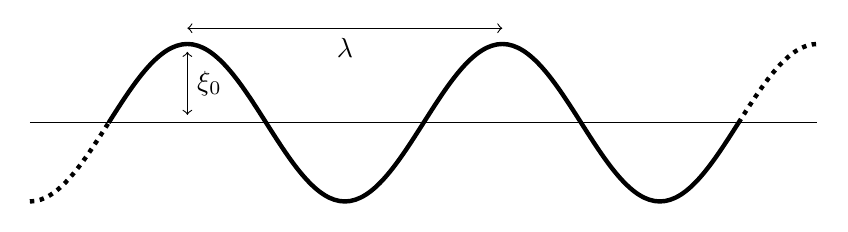
\begin{tikzpicture}

	% Baseline
	\draw (1,0) -- (11,0);

	% Wave
	\draw[x=1cm,y=1cm,dotted,ultra thick] (1,-1) cos (2,0);
	\draw[x=1cm,y=1cm,ultra thick] (2,0)
		sin (3,1) cos (4,0) sin (5,-1) cos (6,0)
		sin (7,1) cos (8,0) sin (9,-1) cos (10,0);
	\draw[x=1cm,y=1cm,dotted,ultra thick] (10,0) sin (11,1);

	% Labels
	\draw[<->] (3,1.2) -- (7,1.2);
	\node[below] at (5,1.2) {$\lambda$};
	\draw[<->] (3,0.1) -- (3,0.9);
	\node[right] at (3,0.5) {$\xi_0$};

\end{tikzpicture}


Ausbreitungsgeschwindigkeit $c$:
\[
	c = \lambda f
\]
Kreisfrequenz $\omega$:
\[
	\omega = \frac{2 \pi}{T}
\]
Wellenzahl $k$:
\[
	k = \frac{2 \pi}{\lambda}
\]
Auslenkung $\xi$ am Ort $x$ zum Zeitpunkt $t$:
\[
	\xi = \xi_0 \sin (\omega t - k x - \varphi_0)
\]
